%%%%%%%%%%%%%%%%%%%%%%%%%%%%%%%%%%%%%%%%%%%%%%%%%%%%%%%%%%%%%%%%%%%%%%
%
% Institut für Rechnergestuetzte Automation
% Forschungsgruppe Industrial Software
% Arbeitsgruppe ESSE
% http://security.inso.tuwien.ac.at/
% lva.security@inso.tuwien.ac.at
%
% Version 2014-04-08
% 
%%%%%%%%%%%%%%%%%%%%%%%%%%%%%%%%%%%%%%%%%%%%%%%%%%%%%%%%%%%%%%%%%%%%%%

\documentclass[12pt,a4paper,titlepage,oneside]{scrartcl}
\usepackage{esseProtocol}
\usepackage{dirtree}
\usepackage{multirow}
\usepackage{bigstrut}

%%%%%%%%%%%%%%%%%%%%%%%%%%%%%%%%%%%%%%%%%%%%%%%%%%%%%%%%%%%%%%%%%%%%%%
%
% FOR STUDENTS
%
%%%%%%%%%%%%%%%%%%%%%%%%%%%%%%%%%%%%%%%%%%%%%%%%%%%%%%%%%%%%%%%%%%%%%%

% Group number or "0" for Lab0
\newcommand{\gruppe}{13}
% Date
\newcommand{\datum}{2014-05-16}
% valid values: "Lab0", "Lab1" (be sure to use Uppercase for first character)
\newcommand{\lab}{Lab1}

% name of course
\newcommand{\lvaname}{Security for Systems Engineering}
% number of course
\newcommand{\lvanr}{183.637}
% year and term, for example: "SS 2012", "WS 2012", "SS 2013", etc.
\newcommand{\semester}{SS 2014}

% Student data in Lab0 or 1. student of group in Lab1
\newcommand{\studentAName}{Ren\'{e} Czerny}
\renewcommand{\studentAMatrnr}{0825750}
\newcommand{\studentAEmail}{e0825750@student.tuwien.ac.at}

% 2. student of group in Lab1, for Lab0 or if your group has less students, remove these 3 lines
\newcommand{\studentBName}{Zoltan Krekus}
\renewcommand{\studentBMatrnr}{0702077}
\newcommand{\studentBEmail}{e0702077@student.tuwien.ac.at}

% 3. student of group in Lab1, for Lab0 or if your group has less students, remove these 3 lines
\newcommand{\studentCName}{Philipp Muhoray}
\renewcommand{\studentCMatrnr}{0967964}
\newcommand{\studentCEmail}{e0967964@student.tuwien.ac.at}

% 4. student of group in Lab1, for Lab0 or if your group has less students, remove these 3 lines
\newcommand{\studentDName}{Peter Neubauer}
\renewcommand{\studentDMatrnr}{0725263}
\newcommand{\studentDEmail}{e0725263@student.tuwien.ac.at}

%%%%%%%%%%%%%%%%%%%%%%%%%%%%%%%%%%%%%%%%%%%%%%%%%%%%%%%%%%%%%%%%%%%%%%
%
% DO NOT CHANGE THE FOLLOWING PART
%
%%%%%%%%%%%%%%%%%%%%%%%%%%%%%%%%%%%%%%%%%%%%%%%%%%%%%%%%%%%%%%%%%%%%%%

\newcommand{\lang}{en}
\newcommand{\colormode}{color}
\newcommand{\dokumenttyp}{Report \lab}

\begin{document}

\maketitle
\setcounter{section}{0}
\setcounter{tocdepth}{2}
\tableofcontents

%%%%%%%%%%%%%%%%%%%%%%%%%%%%%%%%%%%%%%%%%%%%%%%%%%%%%%%%%%%%%%%%%%%%%%
%
% CONTENT OF DOCUMENT STARTS HERE
%
%%%%%%%%%%%%%%%%%%%%%%%%%%%%%%%%%%%%%%%%%%%%%%%%%%%%%%%%%%%%%%%%%%%%%%

\section{Lab1a}

\subsection{Port-Forwarding}

Using the credentials we got at the previous exercise, we could login to the lab environment and from there, we had access to a web server running a web application, which used an old version of the Apache Wicket Framework. This version of Apache Wicket is supposed to have a vulnerability, which we can use to complete the exercise.
The first challenge that presented itself to us was the fact, that we need to access the web application using a browser. But how do you use a browser over ssh? To resolve the issue, we used port forwarding:

\begin{lstlisting}[style=simple]
ssh -N e0825750@tese.inso.tuwien.ac.at -p 15000 -L 8989:10.10.20.100:8080
\end{lstlisting}

All the traffic that goes to the port 8989 is now redirected to 10.10.20.100 on Port 8080. As this is where the web application lies, we can enter

\begin{lstlisting}[style=simple]
http://localhost:8989/login/
\end{lstlisting}

in a browser to access the web application.

\newpage
\subsection{Exploiting the Vulnerability}
The next step was to find a suitable vulnerability for this Apache Wicket version. A look at the the source code revealed the version of the framework (Apache Wicket 1.5.4). A little bit of trying and getting the website to know, we discovered an information revealing comment in the source code after trying to login with invalid credentials:

\begin{lstlisting}[style=simple]
- - - - - - - - - - - - - - - - - - - - - - - - - - - - - -
Unhandled Exception:
at.ac.tuwien.inso.MatchingUserNotFoundException: Couldn't find the given user in file:/var/lib/tomcat7/webapps/login/WEB-INF/classes/at/ac/tuwien/inso/EsseCorp/users.xml
- - - - - - - - - - - - - - - - - - - - - - - - - - - - - -
\end{lstlisting}

This indeed told a lot about the web application's structure.

Our next step brought us to a huge vulnerability database, where we searched for relevant vulnerabilities and maybe even exploits (\emph{http://www.cvedetails.com}). We found a very useful directory traversal vulnerability (\emph{CVE-2012-1089 - http://www.cvedetails.com/cve/CVE-2012-1089/}), which combined with the knowledge about the users.xml from above should prove useful.

The part that really took time and nerves was trying to use the vulnerability. We searched what felt like the whole internet for a clearer description than \emph{"Directory traversal vulnerability in Apache Wicket 1.4.x before 1.4.20 and 1.5.x before 1.5.5 allows remote attackers to read arbitrary web-application files via a relative pathname in a URL for a Wicket resource that corresponds to a null package."}, but didn't manage to find one. Here we learnt an important lesson. Exploiting takes a good deal of patience, trial-and-error and "don't give up".
in the end we managed to find the users.xml file by accessing the following address:

\begin{lstlisting}[style=simple]
http://localhost:8989/login/wicket/resource/at.ac.tuwien.inso.EsseCorp.Login/users.xml
\end{lstlisting}

There we got the second part of the password. The first part could be found in \emph{group.txt} in our home directory on the lab environment.
Now we were able to logon via ssh using the password \emph{soocheenooquaul}.

\begin{lstlisting}[style=simple]
ssh user13@10.10.20.100
\end{lstlisting}

\section{Lab1b}

\subsection{Host Discovery and Name Resolution}
The first step to explore the network is to find out which hosts can be found in the networks to scan. To find out which network we are in, we can use the command

\begin{lstlisting}[style=simple]
user13:$ /sbin/ifconfig 
\end{lstlisting}

So we discover, that we are in the network \emph{192.168.98.0/24}. This gives us a good hint where to scan, additionally to the exercise description:

\begin{lstlisting}[style=simple]
user13:$ nmap -sn 192.168.0.0/16
user13:$ nmap -sn 172.16.0.0/16
\end{lstlisting}

The results are as follows:

\begin{tabular}{l | l}
\hline
192.168.98.1 & omega.local.vienna.essecorp.invalid \bigstrut \\ \hline
192.168.98.10 & alpha.local.vienna.essecorp.invalid \bigstrut \\ \hline
192.168.98.28 & beta.local.vienna.essecorp.invalid \bigstrut \\ \hline
192.168.98.54 & gamma.local.vienna.essecorp.invalid \bigstrut \\ \hline
192.168.98.99 & delta.local.vienna.essecorp.invalid \bigstrut \\ \hline
192.168.98.124 & tomcat.local.vienna.essecorp.invalid \bigstrut \\ \hline
192.168.98.201 & epsilon.local.vienna.essecorp.invalid \bigstrut \\ \hline
192.168.98.202 & zeta.local.vienna.essecorp.invalid \bigstrut \\ \hline
172.16.2.12 & gemini.dmz.vienna.essecorp.invalid \bigstrut \\ \hline
172.16.2.15 & phoenix.dmz.vienna.essecorp.invalid \bigstrut \\ \hline
172.16.2.25 & taurus.dmz.vienna.essecorp.invalid \bigstrut \\ \hline
172.16.2.253 & lyra.dmz.vienna.essecorp.invalid \bigstrut \\ \hline
\end{tabular}

In order to detect the IPv6 addresses of the found domains we use the fact that nslookup also lists IPv6 addresses for given domains, if we set the type to AAAA:

\begin{lstlisting}[style=simple]
user13:$ nslookup 
>set type=AAAA
alpha.local.vienna.essecorp.invalid
...
\end{lstlisting}

Here are the resulting IPv6 addresses:

\begin{tabular}{l | l}
\hline
omega.local.vienna.essecorp.invalid & fdcb:c447:e9d2:3553:1001::1 \bigstrut \\ \hline
alpha.local.vienna.essecorp.invalid & fdcb:c447:e9d2:3553:1001::5 \bigstrut \\ \hline
beta.local.vienna.essecorp.invalid & fdcb:c447:e9d2:3553:1001::9 \bigstrut \\ \hline
gamma.local.vienna.essecorp.invalid & fdcb:c447:e9d2:3553:1001::21 \bigstrut \\ \hline
delta.local.vienna.essecorp.invalid & fdcb:c447:e9d2:3553:1001::43 \bigstrut \\ \hline
tomcat.local.vienna.essecorp.invalid & fdcb:c447:e9d2:3553:1001::ab \bigstrut \\ \hline
epsilon.local.vienna.essecorp.invalid & fdcb:c447:e9d2:3553:1001::79 \bigstrut \\ \hline
zeta.local.vienna.essecorp.invalid & fdcb:c447:e9d2:3553:1001::88 \bigstrut \\ \hline
lyra.dmz.vienna.essecorp.invalid & fdcb:c447:e9d2:3553:1002::fd \bigstrut \\ \hline
\end{tabular}

But what about the IPv6 hosts, who are IPv6-only and have therefore not yet been discovered? Unfortunately nmap does not provide the possibility to scan ranges of IPv6 addresses, which is why we have to create our own ping script and let it run for every subnet in the exercise description (\emph{fdcb:c447:e9d2:3553:1000::} to \emph{fdcb:c447:e9d2:3553:100f::}):

\begin{lstlisting}[style=simple]
for i in `seq 1 255`; do i=$(printf "%x" $i); echo "Trying $i..."; ping6 -c 1 -t 1 "fdcb:c447:e9d2:3553:1000:0000:0000:00$i" > /dev/null && echo "Host $i is running"; done
\end{lstlisting}

However, no additional hosts have been found using this method.

\subsection{MAC addresses}

The MAC addresses have been obtained by looking at the ARP table, and at the information about the own network interfaces. The addresses not currently in the ARP table can be forced into it by simply pinging the required host.

\begin{lstlisting}[style=simple]
user13:$ cat /proc/net/arp | grep 192.168
user13:$ /sbin/ifconfig
\end{lstlisting}

The results are the MAC addresses, which reside in the same subnet.

\begin{tabular}{l | l}
\hline
192.168.98.1 & 00:1b:d2:0d:84:98 \bigstrut \\ \hline
192.168.98.10 & 00:1b:d2:d1:1f:85 \bigstrut \\ \hline
192.168.98.28 & 00:1b:d2:f0:60:59 \bigstrut \\ \hline
192.168.98.54 & 00:1b:d2:83:b8:41 \bigstrut \\ \hline
192.168.98.99 & 00:1b:d2:a7:8f:d2 \bigstrut \\ \hline
192.168.98.124 & 00:1b:d2:11:3c:dd \bigstrut \\ \hline
192.168.98.201 & 00:1b:d2:38:ae:b9 \bigstrut \\ \hline
192.168.98.202 & 00:1b:d2:85:9c:c4 \bigstrut \\ \hline
\end{tabular}

\newpage
\subsection{Operating Systems, Ports and Services}

Nmap also has the possibility to guess operating systems and services behind open ports. Sometimes even version numbers. We used the following commands to gain this information. Regarding the operating system, one can also sometimes guess it looking at the services running. Some only run on Unix systems, for example.

\begin{lstlisting}[style=simple]
user13:$ nmap -A 192.168.98.1/24
user13:$ nmap -A 172.16.2.1/24
\end{lstlisting}

\begin{tabular}{l | l}
\hline
\multirow{2}{*}{192.168.98.1} & OS: Linux (Debian kind) \bigstrut \\ & 22: SSH - OpenSSH 6.0p1 \bigstrut \\ \hline
\multirow{2}{*}{192.168.98.10} & OS: Unix \bigstrut  \\ &  53: DNS - dnsmasq 2.62 \bigstrut \\ \hline
\multirow{4}{*}{192.168.98.28} &OS: Unix \bigstrut \\ & 25: SMTP - Exim smtpd 4.80 \bigstrut \\ & 110: POP3 - Dovecot pop3d \bigstrut \\  & 143: IMAP - Dovecot imapd \bigstrut \\ \hline
\multirow{2}{*}{192.168.98.54} & OS: \bigstrut \\ & 1080: SOCKS - socks5 \bigstrut \\ \hline
\multirow{2}{*}{192.168.98.99} & OS: Unix \bigstrut \\ & 631: IPP - CUPS 1.5 \bigstrut \\ \hline
\multirow{2}{*}{192.168.98.124} & OS: Linux \bigstrut \\ & 8080: HTTP - Apache Tomcat JSP engine 1.1 \bigstrut \\ \hline
\multirow{3}{*}{192.168.98.201} & OS: Unix \bigstrut \\ & 139: netbios-ssn - Samba 3.6.6 \bigstrut \\ & 445: microsoft-ds - Samba 3.6.6 \bigstrut \\ \hline
192.168.98.202 & all ports closed  \bigstrut \\ \hline
\multirow{2}{*}{172.16.2.12} & OS: Unix \bigstrut \\ & 80: HTTP - lighttpd 1.4.31 \bigstrut \\ \hline
\multirow{2}{*}{172.16.2.15} & OS: Unix \bigstrut \\ & 21: FTP - vsftpd 2.3.5 \bigstrut \\ \hline
\multirow{2}{*}{172.16.2.25} & OS: Unix \bigstrut \\ & 25: SMTP - smtpd 4.8 \bigstrut \\ \hline
\multirow{2}{*}{172.16.2.253} & OS: Linux \bigstrut \\ & 22: SSH - OpenSSH 6.0p1 \bigstrut \\ \hline
\end{tabular}

\newpage
\subsection{Functionality}
The functionality can, of course, only be guessed. However the services provided on the servers give a strong hint to what it might be used for. Also nslookup can be used to guess which computers are probably routers (see Network Topology section).
 
\begin{tabular}{l | l}
\hline
192.168.98.1 & router \bigstrut \\ \hline
192.168.98.10 & name server (DNS) \bigstrut \\ \hline
192.168.98.28 & mail server \bigstrut \\ \hline
192.168.98.54 & proxy server \bigstrut \\ \hline
192.168.98.99 & printer server \bigstrut \\ \hline
192.168.98.124 & web application server \bigstrut \\ \hline
192.168.98.201 & file server \bigstrut \\ \hline
192.168.98.202 & unknown \bigstrut \\ \hline
172.16.2.12 & web server \bigstrut \\ \hline
172.16.2.15 & FTP server \bigstrut \\ \hline
172.16.2.25 & mail server (only sending - probably for the tomcat server) \bigstrut \\ \hline
172.16.2.253 & router \bigstrut \\ \hline
\end{tabular}

\subsection{Network Topology}
To discover the network topology, we used trace path, where you can find out which hops a packet needs to pass in order to get to a destination.

\begin{lstlisting}[style=simple]
user13:$ tracepath 172.16.2.12
1:  tomcat.local.vienna.essecorp.invalid                  0.100ms pmtu 1500
1:  omega.local.vienna.essecorp.invalid                  0.721ms 
1:  omega.local.vienna.essecorp.invalid                  0.542ms 
2:  gemini.dmz.vienna.essecorp.invalid                   1.128ms reached
     Resume: pmtu 1500 hops 2 back 63 
\end{lstlisting}

\begin{figure}[h!]
  \centering
  \fbox{
    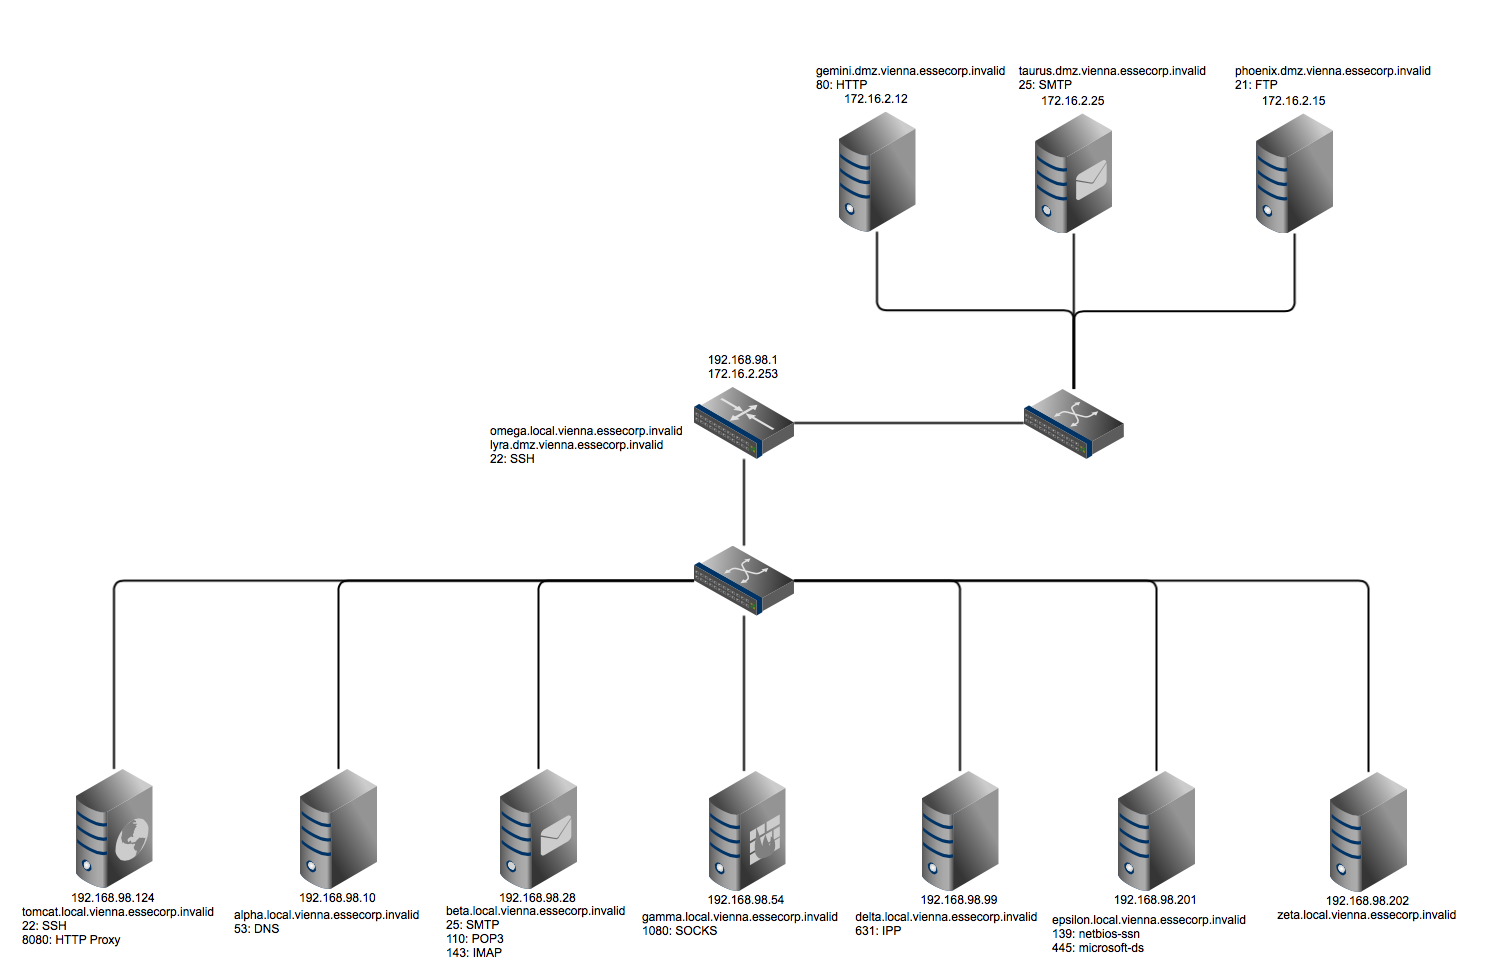
\includegraphics[angle=270,width=0.9\textwidth]{./imgs/network_topology.png}
  }
  \caption{Network Topology}
\end{figure}

\newpage
\section{Lab1c}

\subsection{A0 - XSS (Cross-Site Scripting)}

XSS ist eine Art von Injection. Als signifikantes Merkmal wird der Inhalt der Injection (payload) vom angegriffenen Server an einen oder mehrere Empfänger, die tatsächlichen Angriffsziele, weitergeleitet. Im prominentesten Fall wird die Angriffs-Payload Teil eines HTML-Dokuments, das von einem kompromittierten Webserver an den Browser eines Clients gesendet wird, der eine darauf befindliche Webseite aufruft. Das gleiche Prinzip ermöglicht das Angreifen von E-Mail-Clients, welche E-Mails von einem kompromittierten Server bekommen.

Fehlerquelle
============

Die XSS-Schwäche befindet sich in src-vuln/index.php: Zeile 47-48.
Der String-Inhalt der Datenbank wird durch die Variablen $row[user] und $row[comment] direkt in den HTML-Quellcode der Seite eingebettet. Falls der String nicht nur simplen Text, sondern auch HTML-relevante Information enthält, wird diese zum Teil der Struktur der Webseite. Das ermöglicht dem Angreifer, den Browser von aufrufenden Clients mit allen Anweisungen anzusteuern, die von diesem unterstützt werden, z.B. Javascript.

Ausnutzung
==========

Eingabe eines speziell angefertigten Strings in das 'Text'-Eingabefeld und den Knopf 'Drehen' drücken.
Beispiel: test<script>alert(''hi'')</script>
Der manipulierte String wird nun jedem Aufrufer der Webseite als Teil der Tabelle unter dem Formular zugeschickt.

Behebung
========

Die Abgabelösung in src-fixed/index.php benutzt die PHP-Funktion htmlentities(), um die auszugebenden Strings in ein HTML-kompatibles Format zu konvertieren. Aufrufende Browser interpretieren daraus den korrekten Text, wie er in der Datenbank liegt. Die HTML-Struktur wird nicht beeinträchtigt.

Eine alternative Lösung besteht in der Verwendung eines Objektmodells für die Komponenten der Webseite wie z.B. in .NET. Ein String mit HTML-Entitäten, der einer Web-Komponente als Anzeigetext zugewiesen wird, wird beim Rendering der Komponente 'aufgeräumt'. Der Implementationsaufwand wird vom Web-Programmierer auf das Web-Framework übertragen, was das Fehler-Risiko senkt.

Eine weitere Alternative wäre die Säuberung von Benutzereingaben bereits vor dem Eintragen in die Datenbank, z.B. ebenfalls durch die htmlentities()-Funktion.

Vorkommen in letzter Zeit
=========================

vBulletin:
Die 'private message' Funktion der verbreiteten Webforum-Software vBulletin enthält eine XSS-Schwachstelle, mit der über einen manipulierten Hyperlink beliebiger Code in die Website eingeschleust werden kann.
Als mögliche Konsequenz könnte ein Angreifer unter der Identität des Opfers Aktionen in der Forumsoftware ausführen.
Es handelt sich um einen reflektierten XSS-Angriff, bei dem das Opfer einen manipulierten Link besuchen muss und der Angriffscode nicht am Server gespeichert bleibt.
http://www.cvedetails.com/cve/CVE-2014-3135/
http://packetstormsecurity.com/files/126226/vBulletin-5.1-Cross-Site-Scripting.html (Exploit Beispiel)

phpMyID:
Die Login-Seite von phpMyID, eine identity provider Software für OpenID, kann mittels XSS manipuliert werden. Der Benutzer besucht die anfällige Seite, um sich mit seinen OpenID Credentials einzuloggen. Daher kann jede Webseite, die eine OpenID-Authentifizierung anbietet, einem potentiellen Opfer glaubhaft den XSS-infizierten Link unterschieben. Auch dies ist ein reflektierter XSS-Angriff. Da die Software nicht mehr gewartet wird, bleiben alle bestehenden Deployments verwundbar. Die anfällige Version 0.9 gibt es seit 6 Jahren.
http://www.cvedetails.com/cve/CVE-2014-2890/
http://siege.org/phpmyid (Beschreibung und Dokumentation)

lxml:
Die XML- und HTML-Tool-Library lxml enthält ein Modul zum Aufräumen von HTML-Code. Dieses soll Aufrufe von Javascript entfernen. Allerdings wird ein Aufruf nicht erkannt, wenn die gesuchten Strings wie 'javascript' durch nicht-druckbare Zeichen unterbrochen werden. In der Ausgabe der clean_html()-Funktion befindet sich dann der zusammengesetzte, unerwünschte javascript-Aufruf.
Ein denkbares Anwendungsgebiet dieser Funktion wären Eingabemasken, die einem Benutzer z.B. begrenzte HTML-Eingaben zur Textformatierung ermöglichen. In diesem Fall könnte ein Angreifer die Beschränkungen auf seine Eingabe umgehen.
Die Art der möglichen Angriffe hängt vom Einsatz der lxml-Library ab. Es wäre vorstellbar, dass eine Webseite die Library so einsetzt, dass die 'gesäuberten' Benutzereingaben am Server gespeichert und anderen Benutzern gesendet werden (persistenter XSS-Angriff).
http://cvedetails.com/cve/CVE-2014-3146/
http://seclists.org/fulldisclosure/2014/Apr/319 (Exploit Beispiel)
http://lxml.de/api/lxml.html.clean.Cleaner-class.html (lxml API Dokumentation)

\subsection{A1 - Injection}
This application is a small example of a shell injection vulnerability. Injection in general is a widely distributed vulnerability, which can be used
in various attacks, where one could inject malicious code, get sensitive information, etc.. This example handles a specific version of injection, namely the shell injection. The basis of this vulnerability is, that a user input is forwarded to the system's shell without any validation whatsoever. Attackers can add shell commands to the user input, which will be executed by the program. To counter these attacks, it is necessary to validate the user input, by escaping/removing special characters that are interpreted by the shell, like  \textit{\$, |, \&, <, >, ` and ;}. Even better though, is to completely avoid shell execution from another program, especially if user input is involved.

The example program takes a string as argument and returns it in 1337 speak. It uses the c function
\textit{system(char *string)}, which makes it vulnerable to shell injection (see code line 42 in the vulnerable source code). The fixed program filters
every special character, that could be used in a shell injection and replaces it with an
underscore (see code line 40 and 41 in the fixed source code). Therefore, an attacker is not able to input additional shell commands any more.

The directory structure of the application is as follows:

\dirtree{%
.1 app3. 
.2 exploit. 
.3 Makefile\DTcomment{used to build the example programs}. 
.3 README. 
.2 src-vuln.
.3 1337echo.c\DTcomment{The program vulnerable to shell injection}. 
.2 src-fixed. 
.3 1337echo.c\DTcomment{The program no longer vulnerable to shell injection}. 
}

To compile both the vulnerable and the fixed program, just run

\lstinline{make}

in the \textit{exploit} directory to compile both the vulnerable and the not vulnerable program.

To use the examples after compiling, run 1337echo in the folder \textit{src-vuln} or \textit{src-fixed} (depending on which you want to try):

\lstinline{./1337echo "This is a test!"}

An example exploiting the vulnerability would be (please use with care!):

\lstinline{./1337echo "I will exploit! && rm *"}

An occurrence of a shell injection vulnerability happened in the X.Org X11 server, where remote attackers where allowed to execute commands\footnote{http://www.cvedetails.com/cve/CVE-2011-0465/}. This vulnerability got a CVSS score of 9.3, making it a very delicate one, since it resulted in total information disclosure, total compromise of system integrity and a possibility for total shutdown, while the attacker is not even authenticated.

(\hyperref[code:example1]{see listing~\ref*{code:example1} on page~\pageref*{code:example1}} and \hyperref[code:example2]{see listing~\ref*{code:example2} on page~\pageref*{code:example2}}).

You can include short code snippets or commands directly inline with \lstinline{lstinline block}.

%\lstinputlisting[caption=Example C/C++ file,label=code:example1,style=c]{example.c}

\begin{lstlisting}[caption=Example bash script,label=code:example2,style=simple]
#!/bin/bash
echo "Bash version ${BASH_VERSION}..."
for i in {0..10..2}
  do
     echo "Welcome $i times"
 done

echo "some very very very very very very very very very very very very very very very very very very very very long string"

exit 0;
\end{lstlisting}


%%%%%%%%%%%%%%%%%%%%%%%%%%%%%%%%%%%%%%%%%%%%%%%%%%%%%%%%%%%%%%%%%%%%%%
%
% DO NOT CHANGE THE FOLLOWING PART
%
%%%%%%%%%%%%%%%%%%%%%%%%%%%%%%%%%%%%%%%%%%%%%%%%%%%%%%%%%%%%%%%%%%%%%%

\end{document}


